\chapter{Evaluation}

\section{Usability Evaluation}
{\setstretch{1.9}
Once development of the system had come to a conclusion a usability evaluation was carried out in order to find out how well users interacted with the system. The system is aimed towards members of the Bioschemas and life science communities. These users will likely have varying knowledge and technical abilities, making it vital to design an interface that is as user-friendly and intuitive as possible. For these reasons, members of these communities would have been the ideal test subjects for this evaluation. However, due to logistical issues the ideal test subjects would not be able to participate in A/B testing within a controlled environment. To receive feedback from the ideal test subjects as well as conduct A/B testing to determine the usability of the system, the usability evaluation was carried out in two stages:


{\setstretch{1.7}
\begin{enumerate}
    \item An initial evaluation of the prototype system with the ideal test subjects.
    \item A final evaluation of the complete system with alternate test subjects.
\end{enumerate}
}

\subsection{Prototype Usability Evaluation}\label{sec:prototyUsability}
The prototype usability evaluation subjects consisted of participants from various Bioschemas Meetings\footnote{\url{http://bioschemas.org/meetings/} (accessed 07/03/2019)} that were run by Dr. Alasdair Gray. The evaluation was initially conducted with the first prototype system (Section \ref{ch:prototyping}) that was used to help gathered the initial system requirements and later a second prototype system comparable to the final system (Section \ref{sec:userInterface}) without the additional information panel.

}

The prototype usability test did not consist of a set task. The test subjects were given a demonstration of the prototype and then were given the opportunity to create markup for their own data resource. Once they tested the prototype they were asked to fill out an evaluation questionnaire shown in Appendix \ref{chp:prototypeUsabilityQuestionaire} on various aspects of the system and any additional features they would like to see. This information was then used to improve the final system and tailor it towards the end user. Although useful, the information collected may not be definitive. By not having a set task and control over the conditions the test was conducted in, the resulting information may be affected in comparison to a controlled usability test.

\subsubsection{First Prototype Usability Results}
The prototype usability questionnaire was completed by eleven test subjects. The questionnaire presented test subjects with a total of seven questions. Questions one to four, used a scale, ranging from one to ten, to asses their current knowledge and how they felt about the interface of the prototype. Question five and six, asked the subjects about the information provided and the results. Finally, question seven asked the test subjects to provided written feedback on what features they would like added to the final system. 

As show in Figures \ref{fig:prototypeQuestion1} and \ref{fig:prototypeQuestion2}, the test subjects had a wide range of familiarity with Schema.org and Bioschemas.org, the underlying premise of the system. This information highlighted the necessity to create the final system to be as user-friendly as possible, by providing all the information necessary to use the system without any previous knowledge. \newline 
\begin{figure}[!h]
  \centering
  \begin{minipage}[b]{0.47\textwidth}
    \fbox{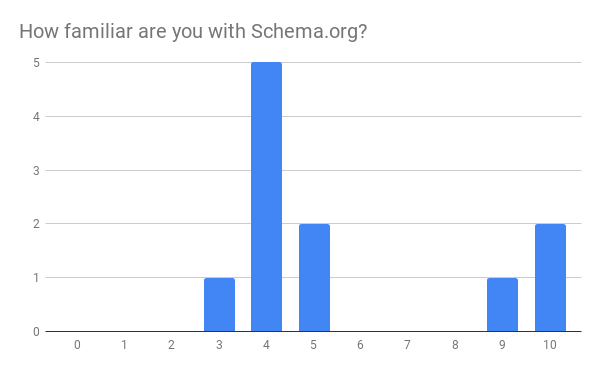
\includegraphics[width=\textwidth]{charts/Prototype/Q1.png}}
\caption{Prototype Evaluation Question 1}
\label{fig:prototypeQuestion1}
  \end{minipage}
  \hfill
  \begin{minipage}[b]{0.47\textwidth}
   \fbox{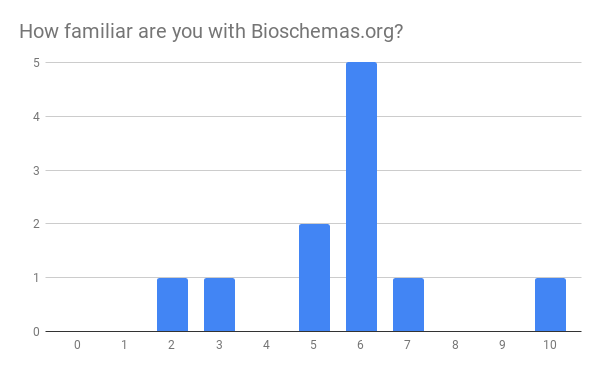
\includegraphics[width=\textwidth]{charts/Prototype/Q2.png}}
\caption{Prototype Evaluation Question 2}
\label{fig:prototypeQuestion2}
  \end{minipage}
\end{figure}

From questions three and four, the overall consensus was that the interface of the prototype was easy to use and appealing, as shown in Figures \ref{fig:prototypeQuestion3} and \ref{fig:prototypeQuestion4}. With the positive reaction of the prototype, the final system was designed using the same layout and appearance. However, a few test subjects commented that they found it difficult to distinguish the marginality of a property (Minimum, Recommend or Optional). Only the minimum properties had a signifier of a small red asterisk next to the property name, but test subjects did not know the meaning of the asterisk until they validated their data. For the final system, this feedback was taken into consideration and a more complete and visible marginality system was implemented. \newline 

\begin{figure}[!h]
  \centering
  \begin{minipage}[b]{0.47\textwidth}
   \fbox{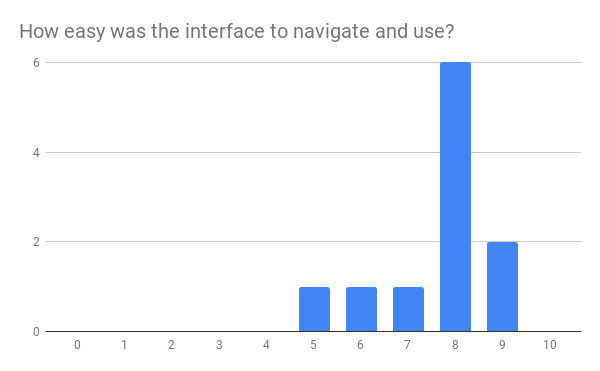
\includegraphics[width=\textwidth]{charts/Prototype/Q3.png}}
    \caption{Prototype Evaluation Question 3}
    \label{fig:prototypeQuestion3}
  \end{minipage}
  \hfill
  \begin{minipage}[b]{0.47\textwidth}
    \fbox{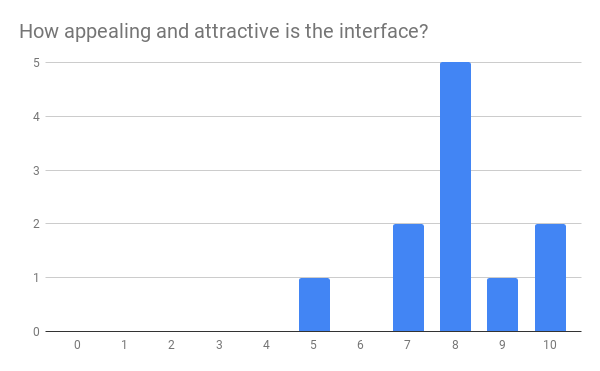
\includegraphics[width=\textwidth]{charts/Prototype/Q4.png}}
    \caption{Prototype Evaluation Question 4}
    \label{fig:prototypeQuestion4}
  \end{minipage}
\end{figure}


{\setstretch{1.7}
Question five had a clear divide in answers from test subjects, as shown in Figure \ref{fig:prototypeQuestion5}. This divide may be due to the nature of the prototype usability test, as test subjects were instructed to create their own markups. This meant test subjects without any personal data or previous knowledge looked for examples to use, but none were provided on the prototype system. For the final system, this feedback was taken into consideration and where possible additional information like examples and controlled vocabularies were provided.\newline
\begin{figure}[!h]
  \centering
  \begin{minipage}[b]{0.47\textwidth}
   \fbox{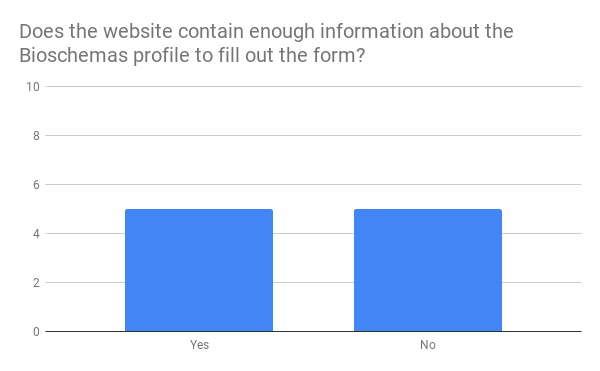
\includegraphics[width=\textwidth]{charts/Prototype/Q5.png}}
    \caption{Prototype Evaluation Question 5}
    \label{fig:prototypeQuestion5}
  \end{minipage}
\end{figure}

Question six asked test subjects if the system generated the expected result from the data users had provided, as shown in Figure \ref{fig:prototypeQuestion6}. In some cases the expected result was unfortunately incorrect. A couple users found that on validation that some properties in the DataCatalog profile were required, but were not actually required in the profiles definition. This was due to human error when manually creating the JSON-Schema to generate the form, as some properties had the required attribute when they should not have. For the final system, these errors will be less likely to occur as the JSON-Schema will be generated directly from the Bioschemas profile without any human intervention. \newline

\begin{figure}[!h]
  \centering
  \begin{minipage}[b]{0.47\textwidth}
   \fbox{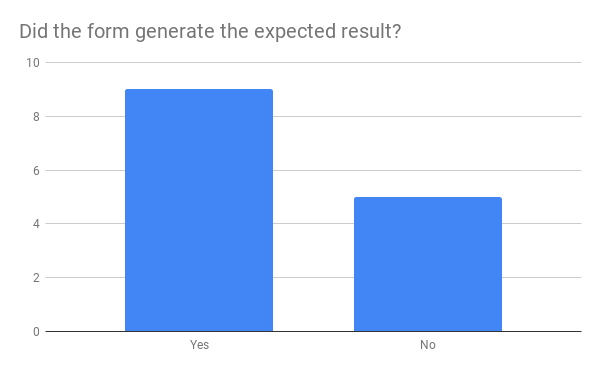
\includegraphics[width=\textwidth]{charts/Prototype/Q6.png}}
    \caption{Prototype Evaluation Question 6}
    \label{fig:prototypeQuestion6}
  \end{minipage}
\end{figure}
}

Question seven asked test subjects if there was any extra features that they would like to see in the final system. This question had overlapping information with the previous questions in which the test subjects stated that they would like to more information to help the users fill out the forms through examples and controlled vocabularies. An additional feature that a test subject requested was to have the resulting data in different formats like RDFa and Microdata, this feature was then included in the system requirements prioritised as a could feature.

In summary, this prototype usability evaluation has been successful in showing that the core functionality and usability of the system works well; although the information provided to the users could be vastly improved. The prototype system was used as a starting platform for the final system and with the feedback provided, the final system was tailored directly towards the end user.  

\newpage
\subsubsection{Second Prototype Usability Results}
The prototype usability questionnaire was completed by two test subjects for the second version of the prototype. The questionnaire presented contained the same questions previously given to test subjects in the first prototype usability evaluation (See Section \ref{sec:prototyUsability}). Unfortunately as only two test subjects completed the questionnaire in which no qualitative feedback was given, no definitive conclusion can be draw to compare the first prototype to the second. From the quantitative data collected, shown in Appendix \ref{chp:prototypeSecondResults}, we can see that test subjects thought the interface was easy to navigate and use and that the prototype was appealing and attractive as well as providing the desired functionality, but these conclusions can not be considered definitive due to the environment in which the usability evaluation was conducted in and the low participation rate.  


\subsection{Final Usability Evaluation}\label{sec:finalUsability}
The final usability evaluation subjects consisted of students from Heriot-Watt University, mainly consisting of students with a Computer Science background. To test the usability of the system developed , a second similar system was used for comparison. In the following sections I will refer to the system developed as \textbf{System A}, which can be seen in Section \ref{sec:userInterface}, and the comparison system as \textbf{System B}, which can be seen in Section \ref{sec:comparisonsystem}.

For each of the systems, the subjects were given a set of tasks to complete. The users were timed for each task, to understand how easily they figured out how to use the systems and any difficulties during the tasks were noted. To eliminate any starting bias towards a system, test subjects alternated between starting on each of systems. Also, to reduce the diversity in times affected by typing speed, test subjects copy and pasted data from the task sheets into each of the systems.

Once the users completed their tasks they were asked to fill out a short questionnaire on each system. This questionnaire asked the users to evaluate various aspects of the system as well as leaving any recommendations to improve the system. The task sheet, questionnaire and consent form signed by the tests subjects can be found in Appendix \ref{chp:finalUsabilityStudy}. 

\subsubsection{Tasks}
Each test subject was assigned the same three tasks for both systems, although an additional task was required for System A. Test subjects will begin Tasks 1, 3 and 4 at the respective Home Page of the system. Task 2 will start where Task 1 left off.

\begin{description}
  \item[Task 1:] Users were asked to markup a DataCatalog profile using the data supplied on their task sheet.
  \item[Task 2:] Users were asked to save the resulting data from Task 1.
  \item[Task 3:] Users were asked to find the Controlled Vocabulary for a property in the Gene profile.
  \item[Task 4:] Users were asked to markup a more complex Gene profile using the data supplied on their task sheet.
\end{description}

\subsubsection{Final Usability Results}\label{sec:finalUsabilityResults}
The final usability test was completed by eight test subjects. The set of the tasks for each system were completed easily by all the test subjects, as reflected by the relatively consistent times taken with the exception of a few outliers, shown in Appendix \ref{sec:taskTimesFinal}. With a faster average task completion time (Shown in Figure \ref{fig:averageTask}) as well as feedback gathered from the questionnaire, it shows that System A was easy to use and was preferred by all test subjects, but could use some minor improvements. \newline

\begin{figure}[!h]
  \centering
  \begin{minipage}[b]{0.6\textwidth}
   \fbox{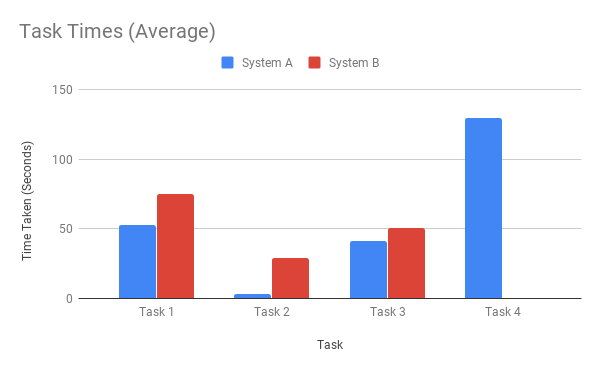
\includegraphics[width=\textwidth]{charts/Average.png}}
    \caption{Average Task Completion Times}
    \label{fig:averageTask}
  \end{minipage}
\end{figure}

\newpage

The questionnaire presented test subjects with a total of seven questions. Questions one to four used a Likert scale, ranging from "Strongly Disagree" to "Strongly Agree", to assess how the subjects felt about each of the interfaces and the amount of information provided by the systems. Additionally, after each question a comment section was also provided to collect any additional information from the test subjects. Question six and seven asked the test subjects to provide written feedback on what could be added to each system or what could be changed. Question eight then asked which system would they prefer to use.

%Question 1 - The interface is easy to use and navigate.
As shown in Figure \ref{fig:finalQ1Bioschemas}, the majority of test subjects considered System A to be easy to use and navigate. The test subject who selected "Neither Agree nor Disagree" left further feedback stating that they found the forms nested design along with the buttons to add and remove items confusing. Two other test subjects also noted that they found the forms buttons to be confusing and another test subject suggested that they should be better separated to help with this issue.

In comparison, only a few test subjects felt that the interface of System B was easy to use, shown in Figure \ref{fig:finalQ1Kaizen}. One test subject stated that they found it easy to use as they already had experience with Google Sheets and were familiar with the interface and layout. However, an issue that was apparent in most evaluations, stemmed from Task Two. Users were asked to save the resulting data from Task One into a HTML file. Users expected that double-clicking would highlight the data to be copied, although in Google Sheets double-clicking shows the user the formula behind the data. This often resulted in test subjects taking multiple attempts to copy to data successfully, increasing the time taken to complete the task, which can be seen in Appendix \ref{sec:taskTimesFinal} with Figures \ref{fig:task2A} and \ref{fig:task2B}.\newline

\begin{figure}[!h]
  \centering
  \begin{minipage}[b]{0.47\textwidth}
   \fbox{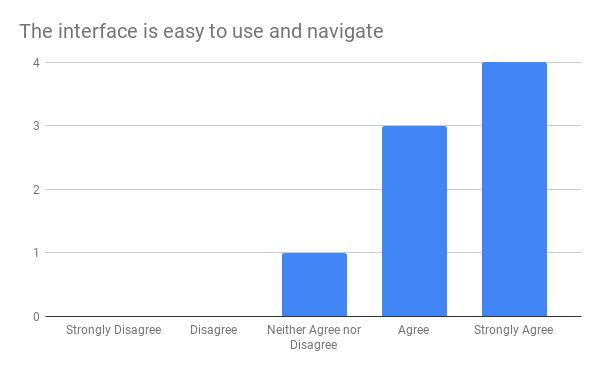
\includegraphics[width=\textwidth]{charts/Final/Bioschemas_The_interface_is_easy_to_use_and_navigate.png}}
    \caption{Question 1: System A}
    \label{fig:finalQ1Bioschemas}
  \end{minipage}
  \hfill
  \begin{minipage}[b]{0.47\textwidth}
    \fbox{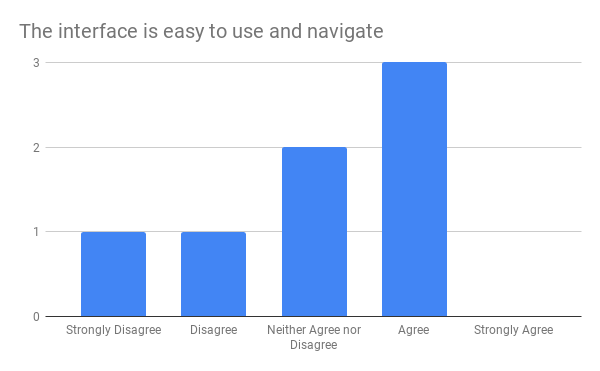
\includegraphics[width=\textwidth]{charts/Final/Kaizen_The_interface_is_easy_to_use_and_navigate.png}}
    \caption{Question 1: System B}
    \label{fig:finalQ1Kaizen}
  \end{minipage}
\end{figure}


\newpage
%Question 2 - The interface is appealing and attractive.%use of graphics. bioschemas %works but poor design. kaizen
Figure \ref{fig:finalQ2Bioschemas} shows that every test subject agreed that they found System A to be aesthetically pleasing. One test subject commented that they liked the flat design of the system but felt that navigation bar could utilise some graphics. Originally, I had intended to use the Bioschemas logo in the navigation bar. Unfortunately, due to selecting the same green for the navigation bar used in the logo, it would have blended in too well and would not have been clearly seen.

In comparison, most test subjects agreed that System B was not aesthetically pleasing, shown in Figure \ref{fig:finalQ2Kaizen}. Two test subjects commented that a separate application would have been a better choice for the design of the interface rather using Google Sheets. Another test subject commented that even though the system was functional, they thought that the system was poorly designed and not aesthetically pleasing. \newline

\begin{figure}[!h]
  \centering
  \begin{minipage}[b]{0.47\textwidth}
   \fbox{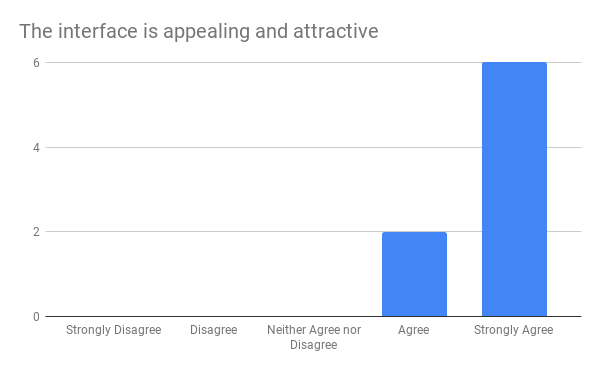
\includegraphics[width=\textwidth]{charts/Final/Bioschemas_The_interface_is_appealing_and_attractive.png}}
    \caption{Question 2: System A}
    \label{fig:finalQ2Bioschemas}
  \end{minipage}
  \hfill
  \begin{minipage}[b]{0.47\textwidth}
    \fbox{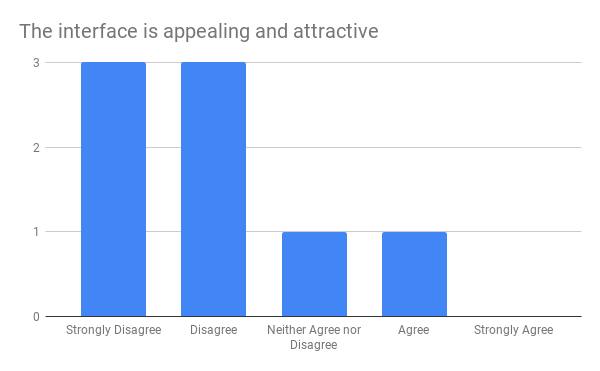
\includegraphics[width=\textwidth]{charts/Final/Kaizen_The_interface_is_appealing_and_attractive.png}}
    \caption{Question 2: System B}
    \label{fig:finalQ2Kaizen}
  \end{minipage}
\end{figure}

%Question 3 - I was able to find the data I needed quickly?
Question three has the most diverse range in answers from test subjects, as shown in Figures \ref{fig:finalQ4Bioschemas} and \ref{fig:finalQ4Kaizen}, which stemmed from Task Three of the usability test. Users were tasked to find the Controlled Vocabulary of a property in the Bioschemas profile Gene.

System A, contained all information necessary to complete Task Three. Although most test subjects found it easy to find the information, some test subjects found it slightly more difficult. One test subject commented that they found the information hard to find as it was hidden within the collapsible sections. To increase the visibility of the information another test subject suggested to label what was contained in the collapsible sections.

\newpage
{\setstretch{1.9}
System B, did not contain the information necessary to complete Task Three, instead it pointed to an external website. A couple test subjects felt that the website that contained information needed was well formatted, but because they had to visit an external website they selected "Neither Agree nor Disagree". Whereas other test subjects felt that they were not able to find the information quickly as they had to visit an external website and disagreed with the question.

\begin{figure}[!h]
  \centering
  \begin{minipage}[b]{0.44\textwidth}
   \fbox{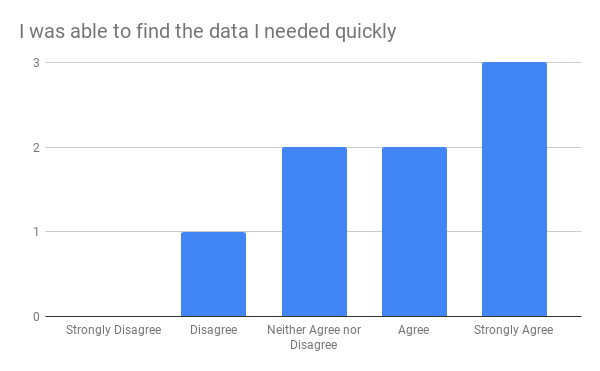
\includegraphics[width=\textwidth]{charts/Final/Bioschemas_I_was_able_to_find_the_data_I_needed_quickly.png}}
    \caption{Question 3: System A}
    \label{fig:finalQ4Bioschemas}
  \end{minipage}
  \hfill
  \begin{minipage}[b]{0.44\textwidth}
    \fbox{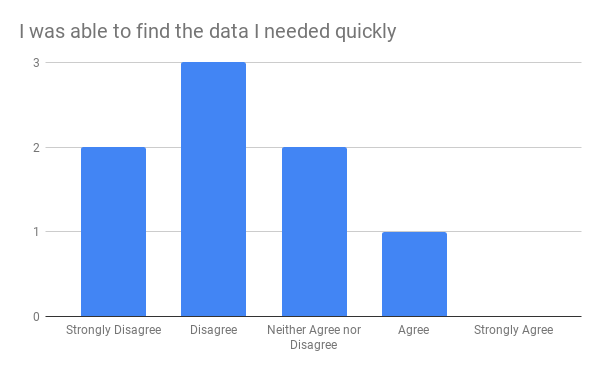
\includegraphics[width=\textwidth]{charts/Final/Kaizen_I_was_able_to_find_the_data_I_needed_quickly.png}}
    \caption{Question 3: System B}
    \label{fig:finalQ4Kaizen}
  \end{minipage}
\end{figure}

%Question 4 - The website contains enough relevant information
Figure \ref{fig:finalQ3Bioschemas} shows that every test subject agreed that System A contained enough relevant information, whereas test subjects agree System B did not agree, shown in Figure \ref{fig:finalQ3Kaizen}. The test subjects felt that to complete the tasks provided that all the information should be provided within the system. The results from this question showed this opinion, as System A contained all the information necessary whereas System B pointed to external website.

\begin{figure}[!h]
  \centering
  \begin{minipage}[b]{0.44\textwidth}
   \fbox{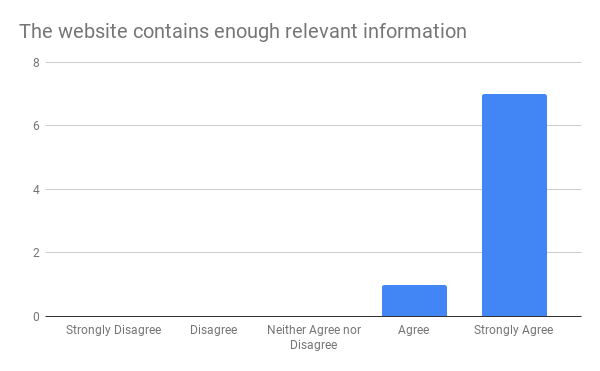
\includegraphics[width=\textwidth]{charts/Final/Bioschemas_The_website_contains_enough_relevant_information.png}}
    \caption{Question 4: System A}
    \label{fig:finalQ3Bioschemas}
  \end{minipage}
  \hfill
  \begin{minipage}[b]{0.44\textwidth}
    \fbox{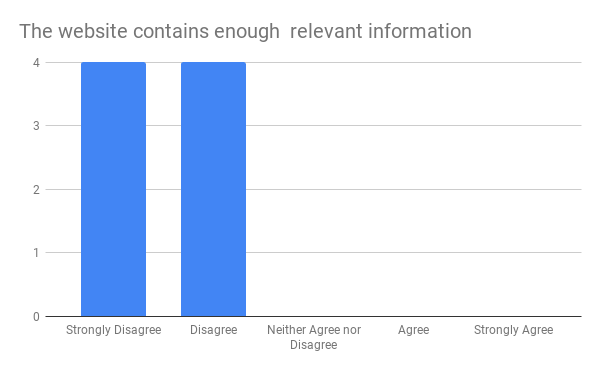
\includegraphics[width=\textwidth]{charts/Final/Kaizen_The_website_contains_enough_relevant_information.png}}
    \caption{Question 4: System B}
    \label{fig:finalQ3Kaizen}
  \end{minipage}
\end{figure}

Question five asked test subjects "Is there anything that you would change about the system?". For System A, test subjects reiterated that they found the forms nested design along with the add item to be confusing and would like these features to be redesigned to be more user friendly. For System B, test subjects reiterated that they would have preferred a separate application to Google Sheets and commented that they would like all the information required to be available and not point to an external website.

}

\newpage
Question six asked test subjects "Is there anything that you like to add to the system?". For System A, only one test subject suggested an addition. Their suggestion was to add graphical feedback when performing actions on the form. For example, when an item is added the area behind the item could change colour letting the user know where the item was added. For System B, a couple test subjects suggested that they would like a feature to easily download the resulting data to a HTML, like in System A.

%Question 7 - Which system did you prefer?
In Summary, this final usability evaluation has been successful in comparing the functionality and the usability of the final system (\textbf{System A}) against a similar system (\textbf{System B}). We can see from Figure \ref{fig:finalQ8} and previous questions, that the test subjects preferred to use system A as it was easy to use, more aesthetically pleasing and provided all the information where necessary; although labelling the information provided could be improved to better the visibility.\newline

\begin{figure}[!h]
  \centering
  \begin{minipage}[b]{0.47\textwidth}
   \fbox{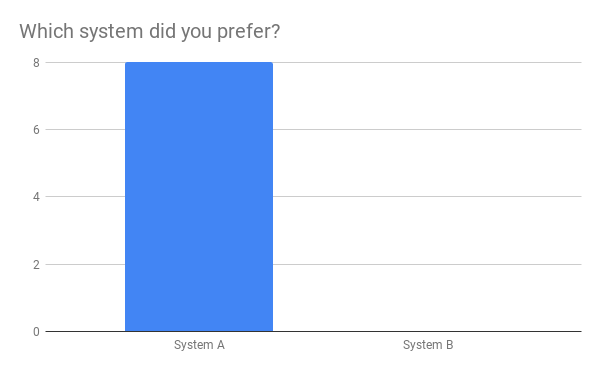
\includegraphics[width=\textwidth]{charts/Final/Which_system_did_you_prefer.png}}
    \caption{Question 7: System A vs System B}
    \label{fig:finalQ8}
  \end{minipage}
\end{figure}


\subsection{Summary of Usability Evaluation}
To summarise, both the final and prototype evaluation were successful in showing that the systems provided the desired functionality outlined at the beginning of the project. It also highlighted the design of the systems were successful in providing an effective, intuitive and aesthetically pleasing user interface and thus test subjects preferred System A over System B. Feedback given during the prototype evaluation was used to further refine the final system towards the target user and feedback given during the final evaluation has been included as future works in Section \ref{sec:futurework}.


\newpage
\section{Requirements Evaluation}
A requirements evaluation was carried out in order to analyse how many system requirements were implemented in the final system compared to the proposed requirements. The evaluation identified which system requirements were successfully implemented, and which were not, along with a description of what was achieved. 
\subsection{Functional Requirements Evaluation}

FR 1 \textbf{The system must allow users to enter data into the form.}
\begin{itemize}
\item[--] Priority: Must
\item[--] Status: Complete
\item[--] Explanation: The system allows users to enter data through form inputs.
\end{itemize}

\noindent
FR 2 \textbf{The system must generate JSON-LD compliant data.}
\begin{itemize}
\item[--] Priority: Must
\item[--] Status: Complete
\item[--] Explanation: The system generates JSON-LD compliant data as tested by the Google Structured Data Testing Tool.
\end{itemize}
\noindent
FR 3 \textbf{The system must allow users to select the Bioschemas profile.}
\begin{itemize}
\item[--] Priority: Must
\item[--] Status: Complete
\item[--] Explanation: The users can select which Bioschemas profile they would like to generate a markup for through a drop-down list.
\end{itemize}

\newpage
\noindent
FR 4 \textbf{The system must be able to handle Schema.org data types.}
\begin{itemize}
\item[--] Priority: Must
\item[--] Status: Complete
\item[--] Explanation: The form inputs can handle each of the Schema.org data types.
\end{itemize}
\noindent
FR 5 \textbf{The system must be able to handle cardinality and marginality.}
\begin{itemize}
\item[--] Priority: Must
\item[--] Status: Complete
\item[--] Explanation: The system can handle cardinality by requiring the minimum properties and displaying the cardinality next to the property name. It can also handle marginality through the JSON-Editors ability to support arrays of multiple types of objects.
\end{itemize}
\noindent
FR 6 \textbf{The system should generate the forms based on a declarative specification.}
\begin{itemize}
\item[--] Priority: Should
\item[--] Status: Complete
\item[--] Explanation: The system generates the JSON-Schema required to generate the form based on declarative specifications from Bioschemas and Schema.org. 
\end{itemize}
\noindent
FR 7 \textbf{The system should be able to handle recursive properties.}
\begin{itemize}
\item[--] Priority: Should
\item[--] Status: Complete
\item[--] Explanation: The JSON-Editor library used for the form is able to handle the recursive properties.
\end{itemize}

\newpage
\noindent
FR 8 \textbf{The system should be able to prioritise form inputs.}
\begin{itemize}
\item[--] Priority: Should
\item[--] Status: Complete
\item[--] Explanation: The form inputs / properties are prioritised by their marginality. First being minimum, then recommended, then optional. 
\end{itemize}

\noindent
FR 9 \textbf{The system should be able to validate the generated markup against the Bioschemas profile.}
\begin{itemize}
\item[--] Priority: Should
\item[--] Status: Partially
\item[--] Explanation: JSON-Editor allows the form inputs to be validated against the JSON-Schema but due to an unknown issue the validation does not work. As JSON-Schema only validates the structure of the data produced and not the data provided, controlled vocabularies would not be able to be validated. Validation could be done through the Validata tool as it would validate both structure and data provided but currently does not have the functionality to do so.

\end{itemize}
\noindent
FR 10 \textbf{The system should display descriptions of each property, as well as examples.}
\begin{itemize}
\item[--] Priority: Should
\item[--] Status: Complete
\item[--] Explanation: Descriptions of each property are displayed next to the relevant form input. Examples are displayed through the Property Tips section and are displayed as a pop-up modal.
\end{itemize}
\noindent
FR 11 \textbf{The system should display the controlled vocabulary of each property.}
\begin{itemize}
\item[--] Priority: Could
\item[--] Status: Complete
\item[--] Explanation: Control Vocabularies are displayed through the Property Tips Section.
\end{itemize}

\newpage
\noindent
FR 12 \textbf{The system could generate Microdata and RDFa along side JSON-LD.}
\begin{itemize}
\item[--] Priority: Could
\item[--] Status: Complete
\item[--] Explanation: The system generates Microdata and RDFa by converting the generated JSON-LD using the RDF Translator API.
\end{itemize}
\noindent
FR 13 \textbf{The system could allow the user to download the data generated.}
\begin{itemize}
\item[--] Priority: Could
\item[--] Status: Complete
\item[--] Explanation: The user can download a HTML file containing either the generated JSON-LD, Microdata or RDFa.
\end{itemize}
FR 14 \textbf{The system wont be able to dynamically update declarative specifications from an online source.}
\begin{itemize}
\item[--] Priority: Wont
\item[--] Status: Incomplete
\item[--] Explanation: This requirement was not expected to be complete as expected, due to time constraints and is included as a future work.
\end{itemize}

\subsection{Non-Functional Requirements Evaluation}
\noindent
NFR 1 \textbf{The system must be easy to use through a simple user interface.}
\begin{itemize}
\item[--] Priority: Must
\item[--] Status: Complete
\item[--] Explanation: Results from the usability evaluation that the test subjects were happy with the interface and its ease of use, although some minor improvements are needed.
\end{itemize}

\newpage
\noindent
NFR 2 \textbf{The system must be available 24/7.}
\begin{itemize}
\item[--] Priority: Must
\item[--] Status: Complete
\item[--] Explanation: The web application is publicly accessible 24/7, hosted on the Heriot-Watt MACS Student/Development web server.
\end{itemize}
\noindent
NFR 3 \textbf{The system should be accessible through the top internet browsers: Google Chrome, Mozilla Firefox and Apple Safari.}
\begin{itemize}
\item[--] Priority: Should
\item[--] Status: Complete
\item[--] Explanation: The web application is accessible through the top web browsers, tested functionality on all three browsers specified.
\end{itemize}

\noindent
NFR 4 \textbf{The system could have two interfaces. One for standard users. Another for administrative users.}
\begin{itemize}
\item[--] Priority: Could
\item[--] Status: Incomplete
\item[--] Explanation: Due to time constraints, I was not able to implement this requirement but is included as future work.
\end{itemize}

\subsection{Summary of Requirements Evaluation}
All but three of the requirements outlined at the beginning of the project were completed, with only one partially complete and two incomplete. Of the two incomplete requirements, one was a functional requirement that was prioritised as a wont, while the other was non-functional that was prioritised as a could. While not vital for the systems functionality, it would be beneficial for these requirements to be complete, thus they have been included as future development tasks in Section \ref{sec:futurework}.

